In parallel with the development of life, there are many optimization problems in many different fields that need to be solved. Generally, optimization problem-solving methods can be divided into two categories, namely exact methods and approximate ones~\cite{talbi2009metaheuristics, eiben2003introduction}. With exact approaches, the algorithms always guarantee to return the globally optimal solution. However, in most real-world problems, especially ones belonging to NP-Hard class, these methods are considered infeasible due to the computational cost and time being too large. Therefore, the main approach to handle these problems is approximate methods, which can give an acceptable solution in an adequate time. Figure~\ref{fig:methos} shows the main directions in the optimization problem-solving approaches.

\setlength{\intextsep}{3pt}
\renewcommand{\scalefigure}{0.6}
\begin{figure}[htbp]
	\centering
	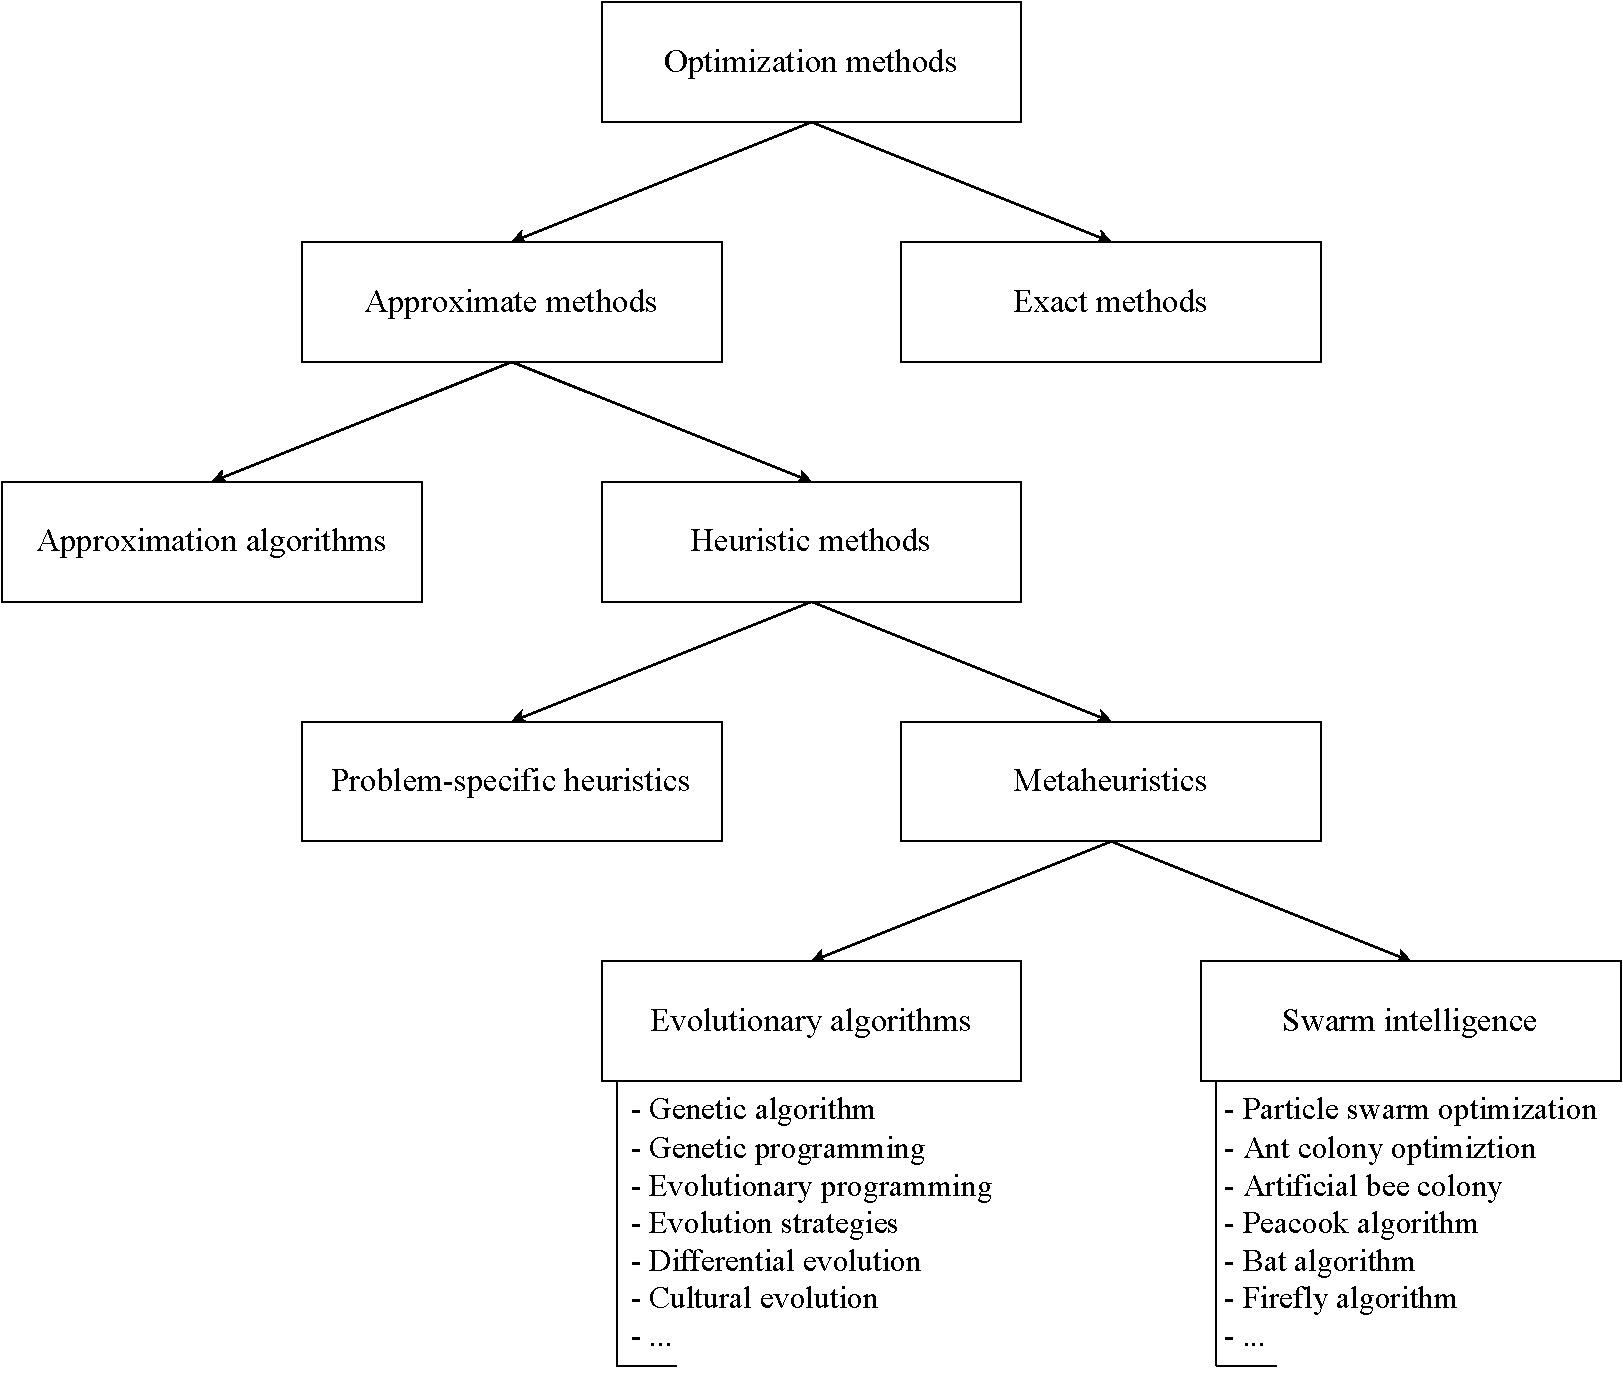
\includegraphics[scale=\scalefigure]{Figures/chap 1/Overview Methods.pdf}
	\caption{Overview of optimization problem-solving methods}
	\label{fig:methos}
\end{figure}

Metaheuristics are known as one method that uses random factors to find the globally optimal solution in the search space. Every metaheuristic algorithm has two major components, i.e., exploration and exploitation~\cite{yang2010nature}. Exploration represents the process of discovering diverse solutions in the search space. Exploitation, on the other hand, is the ability to search locally around an elite solution to improve its quality. Generally, the trade-off between exploration (collecting new information) and exploitation (using existing information) is the main difference between meta-heuristic algorithms. In addition, these components are combined with the selection of the best solutions, which ensures that the solutions will converge to the optimality, while the exploitation via randomization prevents the solutions from being trapped at local optima and, at the same time, increases their diversity. Aside from their simplicity and flexibility, one feature of metaheuristics is that it is independent of the nature of the optimization problem, allowing them to solve any problem merely by following a predetermined general structure of each type of algorithm. Furthermore, this class of algorithms is capable of exploring the entire search space and providing an optimal solution in an acceptable time. With these outstanding advantages, metaheuristics have received more and more attention from the research community over the last few decades.

One most typical class of algorithms of metaheuristics is \gls{ea}. \gls{ea} have as their objective the model of natural evolution, with the core notion is survival of the fittest. By and large, survival is accomplished by reproduction. Offspring from two parents (or more) possess genetic material from both (or all) parents, with the best features of each parent hoped for. Those who inherit negative traits are weak and may lose the battle for survival. Different classes of \gls{ea} have been developed~\cite{engelbrecht2007computational, brabazon2015natural}, including:
\begin{itemize}
	\item \textbf{Genetic algorithm (GA):} model genetic evolution.
	\item \textbf{Genetic programming:} based on \gls{ga}, but individuals are programs (represented as trees).
	\item \textbf{Evolutionary programming:} derived from the simulation of adaptive behavior in evolution (phenotypic evolution).
	\item \textbf{Evolution strategies:} aim to model the strategic parameters that control variation in evolution. 
	\item \textbf{Differential evolution:} similar to genetic algorithms, but differing in the reproduction mechanism used. 
	\item \textbf{Co-evolution:} individuals evolve through cooperation, or in competition with one another, gaining the essential characteristics to survive.
	\item \textbf{Cultural evolution:} model the evolution of a culture of a population and how the culture influences the genetic and phenotypic evolution of individuals. 
\end{itemize}
\gls{ea} has been used successfully in real-world applications, especially NP-hard problems, for example, packet routing, combinatorial optimization, clustering, classification, and scheduling. 

On the other hand, \gls{si} is also a class of metaheuristics that made a wind of change in computational computing. \gls{si} stemmed from the study of colonies, or swarms of social organisms. Thanks to the studies of the social behavior of organisms (individuals) in swarms, the development of highly efficient optimization and clustering algorithms was motivated. Simulations of the elegant, but unexpected, choreography of bird flocks, for instance, led to the development of the Particle Swarm Optimization algorithms~\cite{poli2007particle}, while studies of ant foraging behavior resulted in the design of \gls{aco} algorithms~\cite{parsons2005ant}.